% !TEX TS-program = LuaLaTeX
\documentclass[11pt,compress,xcolor=x11names,UTF8]{beamer}
\usetheme{Singapore}
\usefonttheme{structurebold}
\usecolortheme[named=SpringGreen4]{structure}
% \usepackage{gradientframe} % 图片立体感
\graphicspath{{figure/}} % 图片路径
%% 加入中文
\usepackage[fontset=fandol]{ctex}
% \setCJKsansfont[BoldFont=Noto Sans CJK SC, ItalicFont=Adobe Kaiti Std]{Source Han Serif SC}
% \setsansfont{Roboto}
\usepackage{natbib} % 参考文献
% 数学字体
% \usepackage{mathptm}
% \usepackage{mathptmx}

\title{Spatial Generalized Linear Mixed Models with Application to Prevalence Mapping}
\subtitle{空间广义线性混合模型及其在预测流行病中的应用}
\author{黄湘云 \and XXX}
\institute{
\includegraphics[width=10ex,interpolate=true]{logo} \\~~ \\ 理学院 \\ 中国矿业大学(北京)}
\date{\today}
% \logo{
\includegraphics[width=.15\textwidth]{CUMTB}}
\subject{硕士答辩}
\keywords{混合效应模型}


\begin{document}

\maketitle

\begin{frame}
  \frametitle{内容提要}
  \tableofcontents  
\end{frame}


\section{引言}


\subsection{研究意义}

\begin{frame}{Examples}

\begin{enumerate}
\item radionuclide concentrations on Rongelap Island
\item childhood malaria in the gambia
\item Loa loa prevalence in Cameroon and surrounding areas
\end{enumerate}

\end{frame}

\begin{frame}{Introduction}
\citet{Diggle2002}
\begin{itemize}
\item the effects of child level covariates (age and bed net use)
\item village level covariates (the primary health care and greenness of surrounding vegetation)
\item separate components for residual spatial
\item non-spatial extrabinomial variation
\end{itemize}

$\mathbb{R}^{n}$

$$\log \{p_{ij}/(1-p_{ij})\} =\alpha + \beta'z_{ij} + U_{i} + S(x_{i})$$

\end{frame}

\subsection{文献综述}

\subsection{主要内容}


\section{模型(SGLMM)}

\subsection{模型结构}

\subsection{计算方法}

\subsection{数据分析}

\begin{frame}
\begin{figure}
\centering
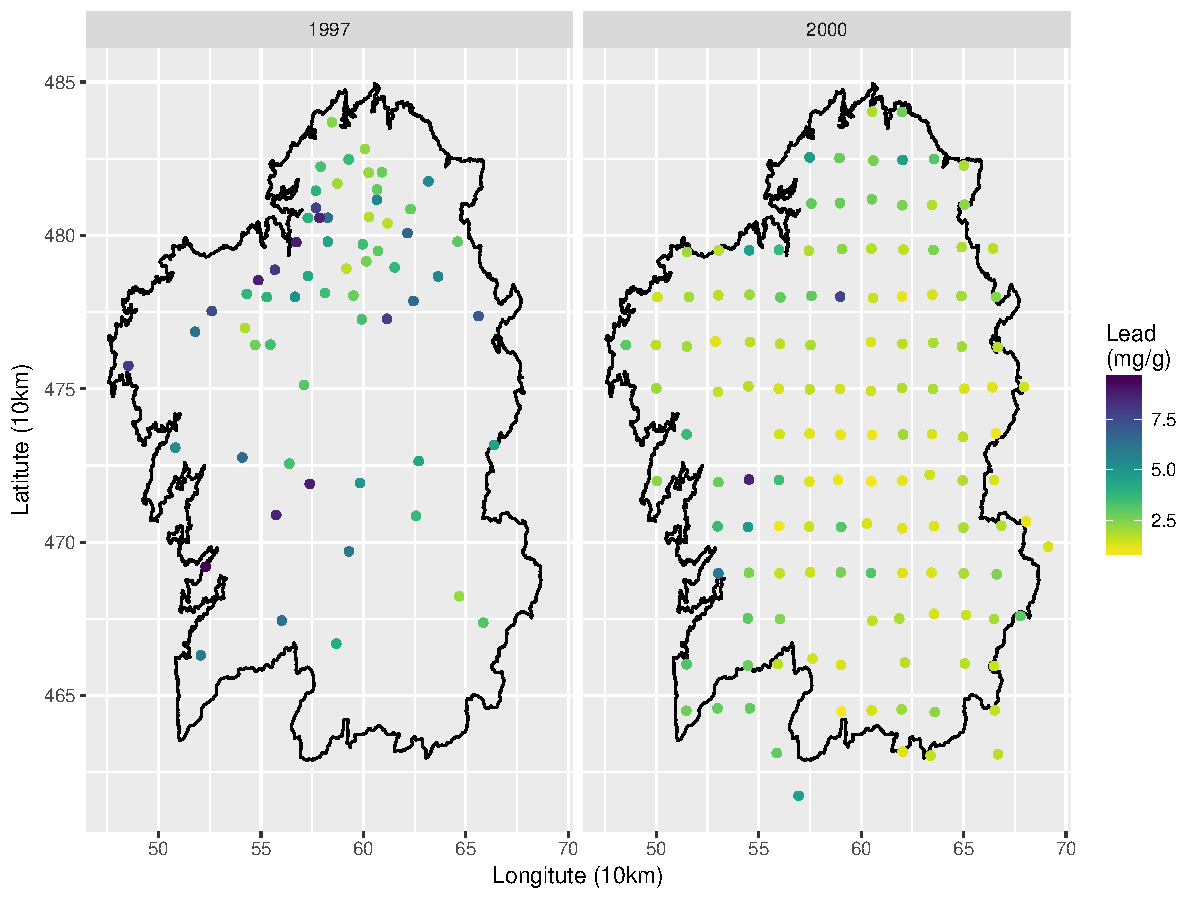
\includegraphics[width=.8\textwidth]{demo03}
\end{figure}
\end{frame}

\section{结论与展望}



\begin{frame}

  \centerline{\Huge\color{red} 谢谢! }

\end{frame}



\begin{frame}[allowframebreaks]
\frametitle{参考文献}
\bibliographystyle{authordate1}
\bibliography{R-GLMM-pkgs}
\end{frame}

\end{document} 


